\chapter{Day 4: Linear Systems of Algebraic Equations}

\section{Schedule}
\begin{itemize}
\item 0900-0915: Debrief
\item 0915-1000: Synthesis
\item 1000-1030: Applications of LSAE
\item 1030-1045: Coffee
\item 1045-1115: Applications of LSAE 
\item 1115-1200: Concept Map for Eigenfaces
\end{itemize}

\section{Debrief}
\bi
\item Please discuss your overnight work with your table-mates, create a set of key concepts, and a set of ideas that you are still confused by.
\ei

\section{Synthesis}

We will increasingly use a computational tool like MATLAB to compute determinants, matrix inverses, and the solutions to linear systems of algebraic equations. In this synthesis section we will explore the theoretical foundation of these algorithms - the so-called LU decomposition. 

\subsection{Gaussian Elimination}

The basic process of \textit{ elimination of variables} can be formalized and is known as Gaussian Elimination. Here will briefly introduce it but you can consult other sources, such as the \textit{Gaussian Elimination} page at WolframMathWorld for more details.

Rather than writing equations, we can cast a LSAE in matrix form and perform \textit{Gaussian Elimination} on the augmented matrix $[\A \; \b]$. 

For example, the linear systems of algebraic equations
\begin{eqnarray*}
2 x_1 + 3 x_2 &=& 6 \\
4 x_1 + 9 x_2 &=& 15
\end{eqnarray*}
can be written as the following augmented matrix 
\[ \twobythree{2}{3}{6}{4}{9}{15} \]
Thinking now in terms of rows, we replace the second row with row 2 - 2 row 1 to give
\[ \twobythree{2}{3}{6}{0}{3}{3} \]
This matrix is now in so-called \textit{echelon} form: we can find the solution to the original LSAE by first solving the equation implied by the last row and then back-substituting into the equation implied by the previous row. 

\begin{prob}
\be
\item Set up the augmented matrix for the following example (you will recognise this from the last assignment)
\begin{eqnarray*}
2x_1 + x_2 &=& 13 \\
4x_1 + 3x_2 &=& 33
\end{eqnarray*}
and perform \textit{Gaussian Elimination} to reduce the augmented matrix to \textit{echelon form}. Interpret the resulting system and determine the solution(s).
\ee
\end{prob}

% \subsection{Gauss-Jordan Elimination}

% Gauss-Jordan elimination is an extension of Gaussian Elimination in order to produce a matrix in \textit{reduced row echelon form}. Here we will briefly introduce it but you could consult other sources, such as the \textit{Gaussian Elimination} page at Wikipedia for more details.

% Starting with the matrix in echelon form
% \[ \twobythree{2}{3}{6}{0}{3}{3} \]
% we eliminate the entry in row 1, column 2 by replacing row 1 with row 1 - row 2
% \[ \twobythree{2}{0}{3}{0}{3}{3} \]
% Finally we divide the first row by 2 and the second row by 3 to give
% \[ \twobythree{1}{0}{3/2}{0}{1}{1} \]
% This matrix is now in \textit{reduced row echelon form} and we simply read off the solution. There is an algorithm in MATLAB , \textit{rref}, which will perform Gauss-Jordan elimination for you.

% \begin{prob}
% \be
% \item Set up the augmented matrix for the example from the last exercise and perform \textit{Gauss-Jordan Elimination} to reduce the augmented matrix to \textit{reduced row echelon form}. Check your answer by using \textit{rref}. Interpret the resulting system and determine the solution(s).
% \ee
% \end{prob}

\subsection{LU Decomposition}
The steps used to solve a LSAE using Gaussian Elimination can also be used to \textit{decompose} a matrix into a product of two matrices: a \textit{lower-triangular} matrix $\L$ and an \textit{upper-triangular} matrix $\U$. Here we will briefly introduce it but you could consult other sources, such as the \textit{LU Decomposition} page at WolframMathWorld for more details.

In Gaussian Elimination we execute a set of row operations. In our ongoing example, we replaced row 2 with the result of row 2 - 2 row 1. This action can be neatly represented in terms of a matrix operation. Let's multiply the original matrix equation $\A \x = \b$ with the transformation matrix
\[ \M = \twobytwo{1}{0}{-2}{1} \]
to form $\M \A \x = \M \b$. Note that this transformation leaves row 1 of $\A$ unchanged, and it replaces the row 2 with row 2 - 2 row 1. The product $\M \A$ is therefore an \textit{upper-triangular} matrix $\U$
\[ \U = \twobytwo{2}{3}{0}{3} \]
and the LSAE is now expressed as $\U \x = \M \b$. If we now multiply this expression by $\M^{-1}$  we obtain
\[ \M^{-1} \U \x = \b \]
The inverse of $\M$ is straight-forward to write down because it "undoes" the row operations
\[ \M^{-1} = \twobytwo{1}{0}{2}{1} \]
Notice that this matrix is just a \textit{lower-triangular} matrix $\L$. The LSAE now reads
\[ \L \U \x = \b \]
We have therefore \textit{decomposed} the original matrix $\A$ into the product of $\L$ and $\U$,
\[ \A = \L \U \]
How does this help, you might be asking? First of all, knowing the decomposition of $\A$ into $\L \U$ allows us to solve the original LSAE $\A \x = \b$. Here is how.

Let's define a new vector $\y = \U \x$. Then the original LSAE can be expressed as
\[ \L \y = \b \]
which is straight-forward to solve by \textit{forward-substitution} because $\L$ is \textit{lower-triangular},
\[ \twobytwo{1}{0}{2}{1} \twobyone{y_1}{y_2} = \twobyone{6}{15} \]
and the solution for $\y$ is $y_1 = 6$, $y_2 = 3$. We can now solve $\U \x = \y$ for $\x$ using \textit{ forward-substitution} because $\U$ is \textit{upper-triangular},
\[ \twobytwo{2}{3}{0}{3} \twobyone{x_1}{x_2} = \twobyone{6}{3} \]
and the solution for $\x$ is $x_1 = 1$, $x_2 = 3/2$.

Second of all, and more importantly, knowing the decomposition of $\A$ into $\L \U$ allows us to solve any LSAE involving $\A$. Need to solve the LSAE with a different $\b$? No problem, just use the $\L \U$ decomposition that you already computed and away you go. No need to redo all the steps of \textit{ Gaussian Elimination} just because $\b$ changed. Need to solve a LSAE for lots of different $\b$'s? No problem, just use the $\L \U$ decomposition that you already computed and away you go. Finally, if you want to compute the inverse or determinant of a matrix this is easy too using LU decomposition as we show next. 

There is an algorithm in MATLAB, \textit{lu}, which does LU decomposition for you, but you should not necessarily expect to get the same $\L$ and $\U$, even for this example. (There are a variety of ways to define the $\L$ and $\U$ matrices, but this is beyond the scope of this section.)

\begin{prob}
\be
\item Consider the appropriate matrix from the last exercise and perform \textit{LU Decomposition}. Check your answer by confirming that $\A = \L \U$. (Please note that you perform LU decomposition on the original matrix $\A$, not the augmented matrix.)
\ee
\end{prob}

\subsection{Determinant}

The basic algorithm for computing a determinant of $\A$ is to first perform LU decomposition, and make use of the following property:
\begin{quote}
The determinant of an upper-triangular or lower-triangular matrix is just the product of the diagonal entries.
\end{quote}
We already met another property of determinants, namely that the determinant of a product is just the product of the determinants. Therefore, $det(\A) = det(\L) det(\U)$, each of which is just the product of the diagonal entries.

\begin{prob}
\be
\item Consider the appropriate matrix from the last exercise and find the determinant using the LU decomposition previously determined. Check your answer using \textit{det} in MATLAB.
\ee
\end{prob}

\subsection{Inverse}

The basic algorithm for computing the inverse of $\A$ is to first perform LU decomposition, and make use of the following idea. $\B$ is the inverse of $\A$ if it satisfies the following property
\[ \A \B = \I \]
The columns of $\B$ are just the solutions of a LSAE with a different $\b$. For example, in the two by two case we can solve
\[\A \x = \twobyone{1}{0} \]
and then
\[\A \x = \twobyone{0}{1} \]
and if we fill the columns of $\B$ with the solution to these LSAE we will have constructed the inverse. Since we already have the LU decomposition of $\A$ we simply solve each case using the technique already presented.

For example, the first column of $\B$ is determined as follows: First we solve $\L \y = \b$
\[ \twobytwo{1}{0}{2}{1} \twobyone{y_1}{y_2} = \twobyone{1}{0} \]
to give $y_1 = 1$ and $y_2 = -2$. Now we solve $\U \x = \y$
\[ \twobytwo{2}{3}{0}{3} \twobyone{x_1}{x_2} = \twobyone{1}{-2} \]
and the solution for $\x$ is $x_1 = 3/2$, $x_2 = -2/3$. This is the entries in the first column of the inverse. Repeating this process for $\b = \twobyone{0}{1}$ will give the second column of the inverse which now reads
\[ \A^{-1} = \twobytwo{3/2}{-1/2}{-2/3}{1/3} \]

\begin{prob}
\be
\item Consider the appropriate matrix from the previous exercise and find the inverse using the LU decomposition previously determined. Check your answer using \textit{inv} in MATLAB.
\ee
\end{prob}

\section{Applications of LSAE}

Choose at least one of the following problems involving linear systems of algebraic equations.

\subsection{Truss Analysis}

\begin{prob}
Systems of linear equations often come up in engineering when evaluating the strength and stability of structures under load. A \textit{truss} is a simplified model of a structure. It consists of a collection of straight, rigid elements or sections that are long compared to the dimensions of their cross-section. Sections are connected only at their ends through frictionless, pin joints (Remember them? They can only constrain translation but not rotation, i.e., they can only apply force but not moments to a section). This means that sections of a truss are either in tension or compression (axial forces along its length). The roller can be assumed to be frictionless, and thus only exerts normal force. In analyzing trusses it is often assumed that the  weight of the sections (dead load) is relatively small, and can therefore be neglected. The method of joints is a classic technique for determining the forces acting on all of the sections of a truss that is in static equilibrium. Here are the steps:

\begin{center}
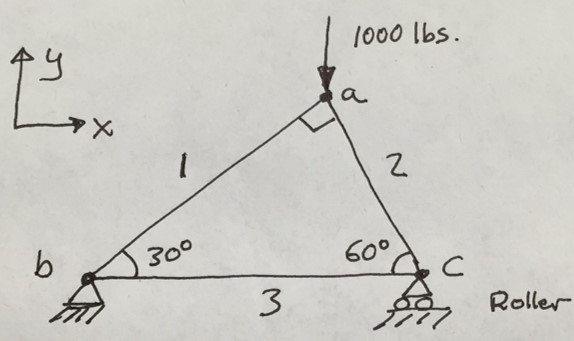
\includegraphics{FacesNight4/figs/triangle1.jpg}
\end{center}

\begin{enumerate}
\item Draw a free body diagram for every pin in the truss. Note that the forces acting at the pin have to be in the directions implied by the things the pin is attached to!
\item  Write out the equations of static equilibrium, $\sum \vec{F} = 0$, for every one of the pins.  Note that some of your forces will be known forces (e.g., external loads), and some will be unknown reaction forces.
\item Express these equations in the matrix form $\A \x  = \mathbf{b}$. 
\item Evaluate whether the system is statically determinate or not.  Note the connection to types of solutions to linear equations here: if you look at the form of $\A$, you should be able to tell whether the system is statically determinate!
\item Find the solution.
\end{enumerate}
\end{prob}
\begin{sol}
\begin{enumerate}
    \item     Note that the pin joint, b, cannot move in space so the ground must apply unknown reaction forces in both the x and y directions. The pin joint, c, is attached to a roller so it is free to move in the x direction but cannot move in the y direction. Therefore, the ground only applies a reaction force (unknown) in the y direction. For the entire truss, there is one known applied external force (1000 lbs) and six unknown axial and reaction forces ($F_1$, $F_2$, $F_3$, $R_{bx}$, $R_{by}$, and $R_{cy}$).
    \begin{center}
        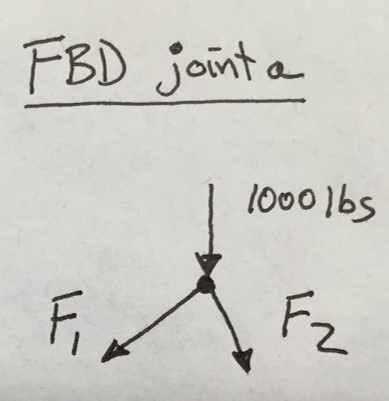
\includegraphics[width=2in]{FacesNight4/figs/trianglea.jpg}
    \end{center}
    \begin{center}
        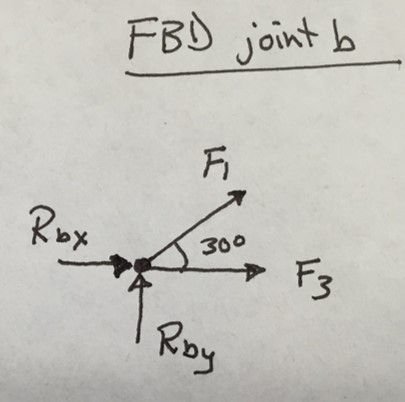
\includegraphics[width=2in]{FacesNight4/figs/triangleb.jpg}
    \end{center}
    \begin{center}
        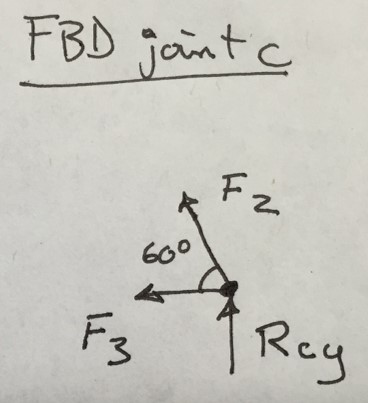
\includegraphics[width=2in]{FacesNight4/figs/trianglec.jpg}
	    \end{center}
	    
	 \item For each joint, $\sum F_x = 0$ and $\sum F_y = 0$. Thus we have the  following six equations:
    \begin{align*}
        -F_1\cos30 + F_2\cos60 &= 0 \\
        -F_1\sin30 - F_2\sin60 &= 1000 \\
        R_{bx} + F_3 + F_1\cos30 &= 0 \\
        R_{by} + F_1\sin30 &= 0 \\
        -F_3 - F_2\cos60 &= 0 \\
        R_{cy} + F_2\sin60 &= 0
    \end{align*}
    
    \item These equations can be written as $\A\x = \mathbf{b}$ where 
    $$\A = \begin{bmatrix}
        -\cos30 & \cos60 & 0 & 0 & 0 & 0 \\
        -\sin30 & -\sin60 & 0 & 0 & 0 & 0 \\
        \cos30 & 0 & 1 & 1 & 0 & 0 \\
        \sin30 & 0 & 0 &  0 & 1 & 0 \\
        0 & -\cos60 & -1 & 0 & 0 & 0 \\
        0 & \sin60 & 0 & 0 & 0 & 1
    \end{bmatrix}, \;$$
    $$\x = \begin{bmatrix} F_1 \\ F_2 \\ F_3 \\ R_{bx} \\ R_{by} \\ R_{cy} \end{bmatrix}$$, \;
    $$\mathbf{b} = \begin{bmatrix} 0 \\ 1000 \\ 0 \\ 0 \\ 0 \\ 0 \end{bmatrix}$$
    
    \item We have 6 unknowns, and 6 equations, so this is a determinate situation.
    
    \item  
        $$\x = \begin{bmatrix}
            -500 \\
            -866.03 \\
            433.01 \\
            -5.6843e^{-14} \\
            250 \\
            750
        \end{bmatrix}$$
    
 Section 3 is the only one in tension ($F_3$ is positive). 1 and 2 should be in compression, and it makes sense that 2 has more compression than 1 because they support the same load, but 2 is more vertical. The horizontal reaction force is $0$ because there is no net horizontal force on the system, and the sum of the vertical reaction forces is $1000\, lbf$ as we expect.
\end{enumerate}
\end{sol}


\subsection{Circuit Analysis}

\begin{prob}
Systems of linear equations naturally arise in circuit analysis, although very few courses on circuits use these anymore. They do, however, form the backbone of circuit design software tools. You've met the relevant physical ideas/models before which are based on Kirchoff's circuit laws: the sum of currents into any node must be zero, and the sum of voltages around any loop must be zero. For the circuit shown in the figure:
\begin{center} 
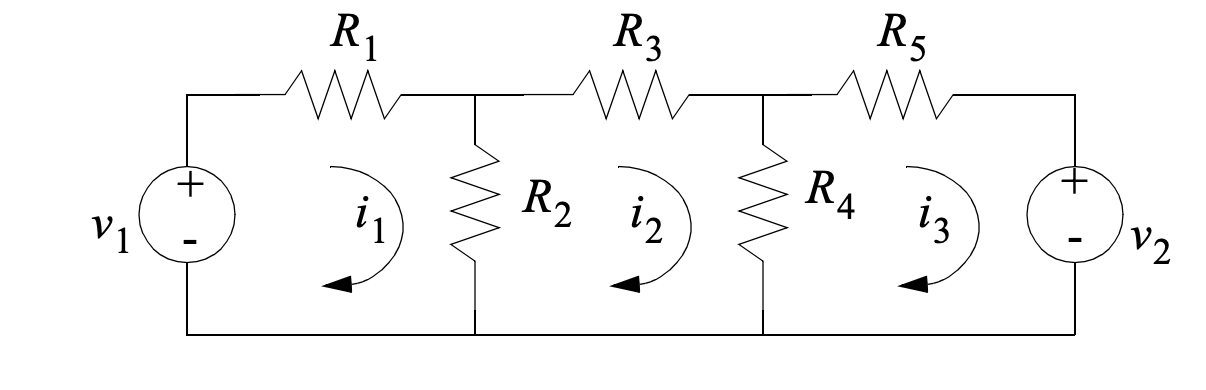
\includegraphics[width=0.75\textwidth]{FacesNight4/figs/simple_circuit.png}
\end{center}

\begin{enumerate}
\item Set up the linear system of algebraic equations required to solve for the three unknown currents (assuming that the resistors and the voltage sources are known.)
\item Find the solution if all of the resistors are 1 ohm, $v_1$ is 5 volts, and $v_2$ is -6 volts.
\end{enumerate}
\end{prob}
\begin{sol}
\begin{enumerate}
    \item  $$\A = \begin{bmatrix}
-R_{1} & -R_{2} & 0 & 0 & 0\\
0 & R_{2} & -R_{3} & -R_{4} & 0\\
0 & 0 & 0 & R_{4} & R_{5}\\
1 & -1 & -1 & 0 & 0\\
0 & 0 & 1 & -1 & 1\\
    \end{bmatrix}, \;$$
    $$\x = \begin{bmatrix} i_1 \\ i_2 \\ i_3 \\ i_4 \\ i_5 \end{bmatrix}$$, \;
    $$\mathbf{b} = \begin{bmatrix} -V_{1} \\ 0 \\ V_{2} \\ 0 \\ 0  \end{bmatrix}$$
    \item $$\x =\begin{bmatrix}
 3.8750\\
    1.1250\\
    2.7500\\
   -1.6250\\
   -4.3750
\end{bmatrix}$$
\end{enumerate}
\end{sol}

\subsection{Chemical Analysis}

\begin{prob}
The complete combustion of propane, $C_3H_8$, with oxygen, $O_2$ yields carbon dioxide, $CO_2$, and water, $H_2O$. Based on conservation of mass, this reaction can be written as
\[a(C_3H_8) + b(O_2) \rightarrow c(CO_2) + d(H_2O)\]
Determine the coefficients in the combustion equation. Note that you will need to learn how to "balance" a chemical reaction.
\end{prob}
\begin{sol}
\[C_3H_8 + 5O_2 \longrightarrow 3CO_2 + 4H_2O\]
\end{sol}

\section{Concept Map for Eigenfaces}

For the facial recognition project we will be primarily focusing on an early facial recognition software algorithm, Eigenfaces, which is still used for face detection, and introduces some other concepts that are extremely important in both facial recognition and other tasks.

We would like you to spend some time developing an understanding of what you know, and what you don't know about facial recognition using Eigenfaces.  A good way to do this is to break down the concept until you get to the point that you have terms that you \textit{do} know:
\be
\item Write the key term at the top or in the center.  Circle it, since you don't know it.
\item Research it, and identify terms that are immediately associated with it.  Write them down and connect them.
\item Circle new terms you don't understand, and break these down too.
\ee

\begin{center}
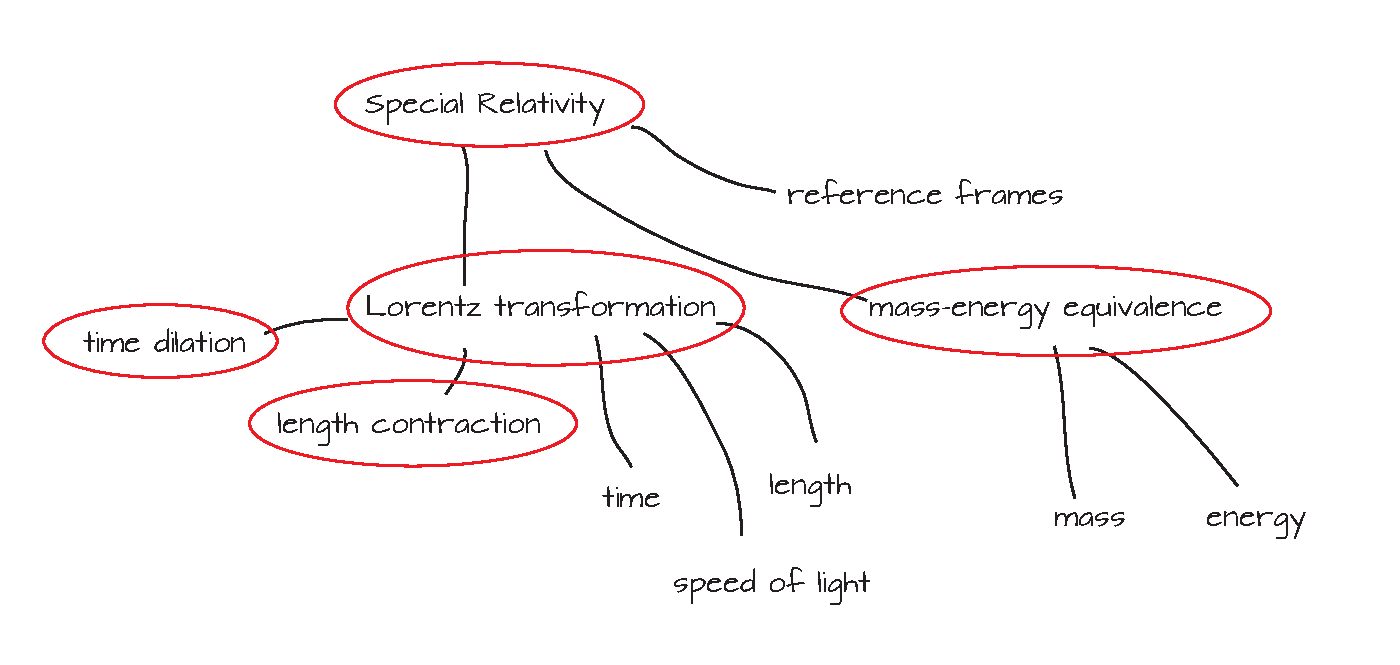
\includegraphics[width=0.75\textwidth]{FacesDay1/figs/ConceptBreakdown.pdf}
\captionof{figure}{If you were trying to break down special relativity, a \textit{portion} of your breakdown might look like this...}
\end{center}

Once you've done your breakdown, try to make the following lists individually:
\be
\item Relevant fundamental mathematical terms that I don't know
\item Relevant fundamental mathematical terms that I do know
\item Ideas specific to facial or image recognition that I don't know
\item Ideas specific to facial or image recognition that I do know
\ee

\pagebreak
\shipoutAnswer
